\documentclass[12pt]{article}

\usepackage{german}
\usepackage[onehalfspacing]{setspace}
\usepackage{graphicx}
\usepackage{float}
\usepackage{subcaption}

\usepackage{geometry}
\geometry{
    left=3cm,
    right=3cm,
    top=2.5cm,
    bottom=2.5cm
}

\usepackage{amsmath}
\usepackage{amssymb}

\begin{document}
\section*{Ausblick}
Für die Herleitung der Weierstraß-Iteration werden wir zuerst die Weierstraß-Iteration der normierten Polynomfunktion
\begin{equation}
  p(x) := x^3+3x^2+2x
\end{equation}
betrachten. Dabei nutzen wir die Startpunkte
\begin{equation}
  z^{(0)}_{1,2,3} := -3, -\frac{-3}{2}, 1
\end{equation}
. Daraufhin werden wir zu einer allgemeinen Herleitung der Weierstraß-Iteration kommen.

\section*{Grundlagen}
Wir haben die allgemeine Form der Weierstraß-Iteration
\begin{equation}
  z_k^{(i+1)} = \frac{p(z_{k}^{(i)})}{\prod_{j=1;j\neq k}^{n}(z_{k}^{(i)}-z_j^{(i)})}
\end{equation}
. Aus dieser können wir die drei Weierstraß-Korrekturterme
\begin{align*}
  z_1^{(i+1)} = \frac{p(z_1^{(i)})}{(z_1^{(i)}-z_2^{(i)})(z_1^{(i)}-z_3^{(i)})}\\
  z_2^{(i+1)} = \frac{p(z_2^{(i)})}{(z_2^{(i)}-z_1^{(i)})(z_2^{(i)}-z_3^{(i)})}\\
  z_3^{(i+1)} = \frac{p(z_3^{(i)})}{(z_3^{(i)}-z_1^{(i)})(z_3^{(i)}-z_2^{(i)})}\\
\end{align*}
bilden. Daraus können wir die drei Korrekturterme der ersten Iteration bilden.
\begin{align*}
  z_1^{(1)} = \frac{p(z_1^{(0)})}{(z_1^{(0)}-z_2^{(0)})(z_1^{(0)}-z_3^{(0)})}\\
  z_2^{(1)} = \frac{p(z_2^{(0)})}{(z_2^{(0)}-z_1^{(0)})(z_2^{(0)}-z_3^{(0)})}\\
  z_3^{(1)} = \frac{p(z_3^{(0)})}{(z_3^{(0)}-z_1^{(0)})(z_3^{(0)}-z_2^{(0)})}\\
\end{align*}
Zunächst werden wir aus diesen Weierstraß-Korrekturen Funktionen bilden, welche den Korrekturwert abhängig von $z_{1,2,3}^{(0)}$ darstellen. Daraufhin werden wir die Weierstraß-Korrekturen in Abhängigkeit von $z_{1,2,3}^{(0)}$ visualisieren.
\begin{align*}
  k_1^{(0)}(z_1^{(0)}) = \frac{p(z_1^{(0)})}{(z_1^{(0)}-z_2^{(0)})(z_1^{(0)}-z_3^{(0)})}\\
  k_2^{(0)}(z_2^{(0)}) = \frac{p(z_2^{(0)})}{(z_2^{(0)}-z_1^{(0)})(z_2^{(0)}-z_3^{(0)})}\\
  k_3^{(0)}(z_3^{(0)}) = \frac{p(z_3^{(0)})}{(z_3^{(0)}-z_1^{(0)})(z_3^{(0)}-z_2^{(0)})}\\
\end{align*}
\begin{figure}[H]
  \centering
  \begin{subfigure}[b]{0.45\textwidth}
    \centering
    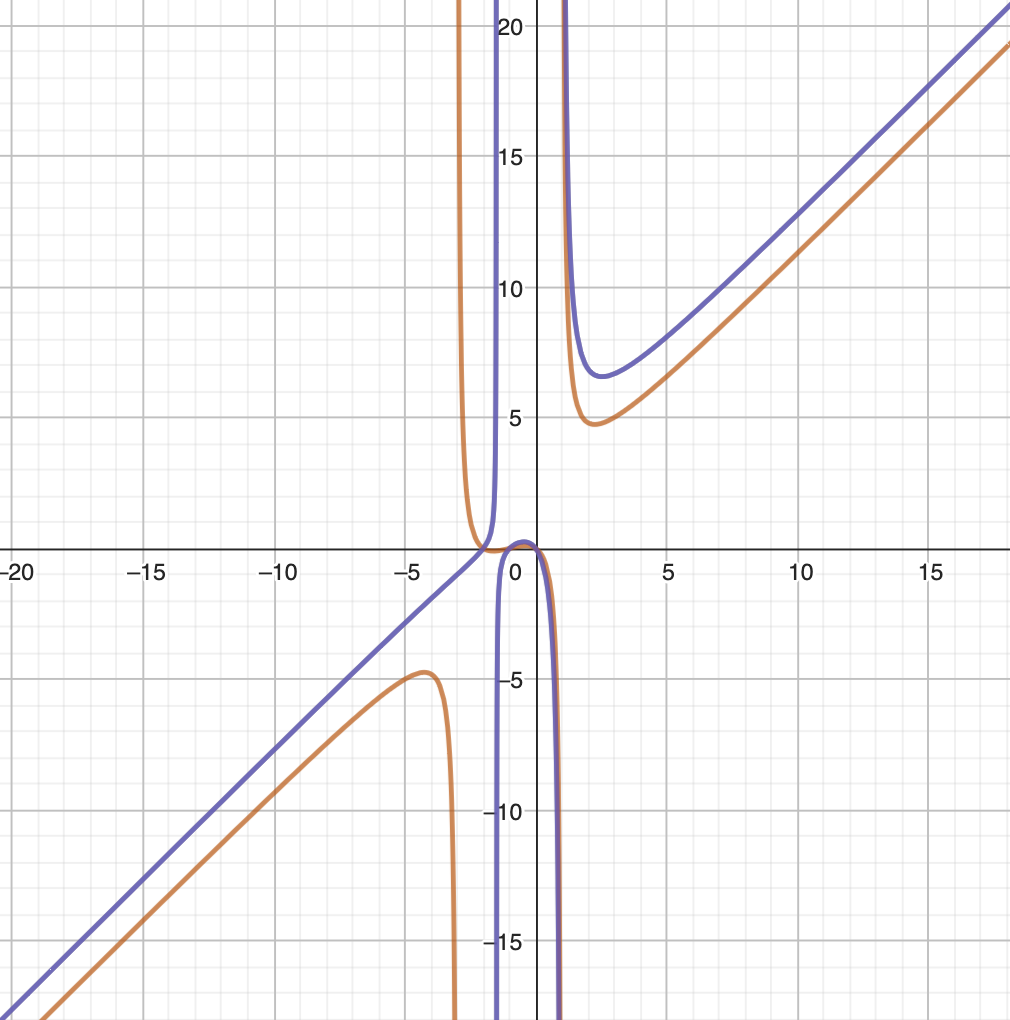
\includegraphics[width=\textwidth]{./Weierstrass_Korrekturen_Far.png}
    \caption{Weierstraß-Korrekturen in Abhängigkeit von $z_{1,2,3}^{(0)}$}
  \end{subfigure}
  \hfill
  \begin{subfigure}[b]{0.45\textwidth}
    \centering
    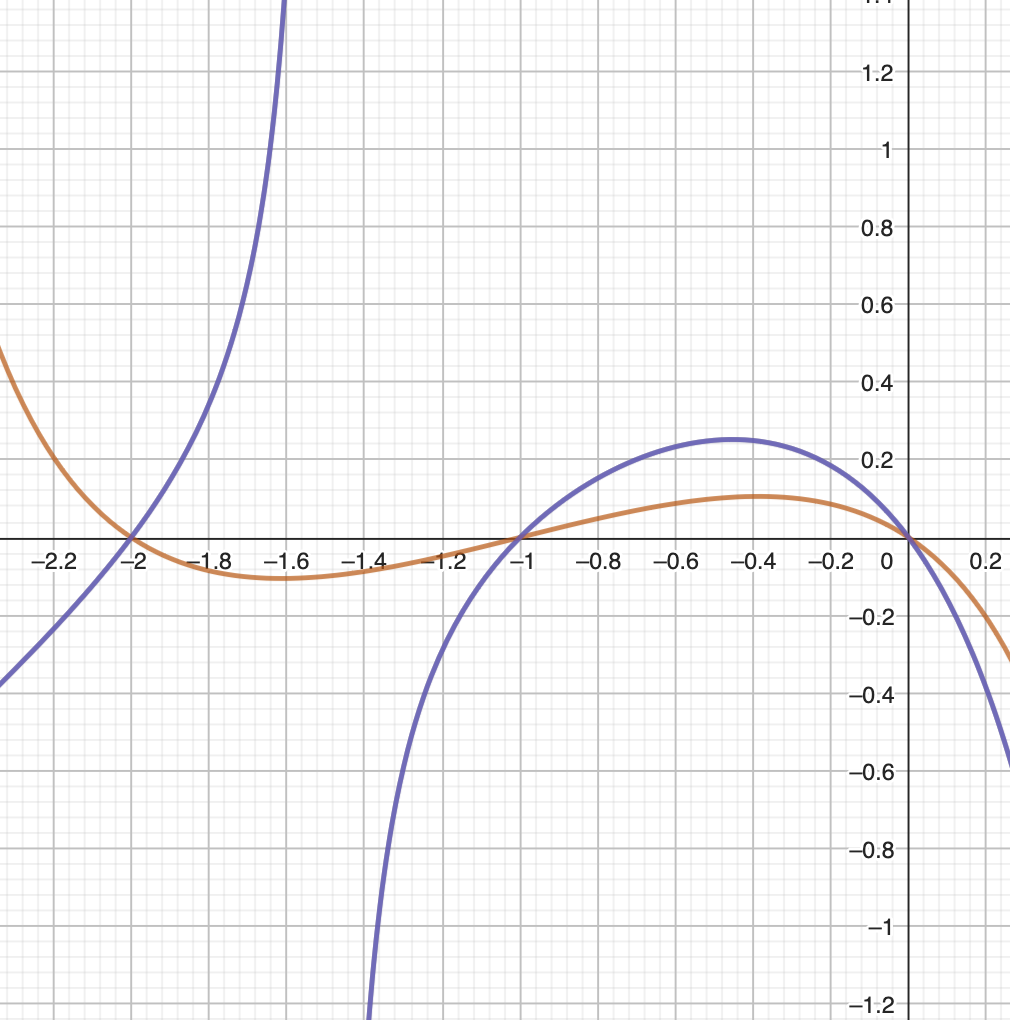
\includegraphics[width=\textwidth]{./Weierstrass_Korrekturen_Close.png}
    \caption{Weierstraß-Korrekturen in Abhängigkeit von $z_{1,2,3}^{(0)}$}
  \end{subfigure}
\end{figure}
Dabei sieht man, dass die Nullstellen der Funktionen $k_{1,2,3}^{(0)}(z_{1,2,3}^{(0)})$ die Nullstellen der Weierstraß-Korrekturen sind. Das lässt sich dadurch erklären, dass der Zähler des Bruches der Weierstraß-Korrektur die Funktion darstellt und auch die gleichen Nullstellen hat. Das bedeutet für die Weierstraß-Iteration, dass der Korrekturterm bei bei den Nullstellen null ist und somit die Iteration bei der Nullstelle bleibt.\\\\
Das ist jedoch nicht der Fall, wenn eine der Nullstellen von $p(x)$ unter $z_j^{(i)}$ mit $j=1,2,3,...,n, j \neq k$ liegt, da in diesem Fall sich auf der Nullstelle eine Definitionslücke befindet.

\paragraph{Schräge Asymptote}
Jede Weierstraß-Korrektur in Abhängigkeit von $z_{1,2,3}^{(0)}$ besitzt eine schräge Asymptote, da der Grad des  Zählerpolynoms eins größer als der Grad des Nennerpolynoms ist. Da das Zählerpolynom normiert ist - also einen Koeffizienten von 1 hat - gilt für die schräge Asymptote $\lim_{x\rightarrow +\infty} k_{1,2,3}^{(0)}(z_{1,2,3}^{(0)}) = +\infty$ und $\lim_{x\rightarrow -\infty} k_{1,2,3}^{(0)}(z_{1,2,3}^{(0)}) = -\infty$. Das heißt, dass sie von dem III. Quadrant in den I. Quadrant verläuft.
\\\\
Im Folgenden werden die Definitionslücken und dazugehörigen Abweichungen von der Asymptote, der einfachheit halbar, nicht berücksichtigt. Diese können den Prozess der Weierstraß-Iteration stören, ändern jedoch nichts an dem eigendlichen Mechanismus hinter der Weierstraß-Iteration. Auf die Definitionslücken und dazugehörigen Abweichungen von der Asymptote wird später eingegangen.
\\\\


\end{document}